\section{引言}
\subsection{问题背景}

华北某山区的乡村地域辽阔，拥有平旱地、梯田、山坡地、水浇地等四类耕地，以及普通大棚和智慧大棚，共54块种植地块、总面积1201.7亩。当地土壤与气候条件多样：平旱地（A1--A6，365亩）适宜小麦、玉米等耐旱作物；梯田（B1--B14，619亩）与山坡地（C1--C6，108亩）以旱作粮食为主；水浇地（D1--D8，109亩）部分种植水稻，其余地块可在第二季复种大白菜、白萝卜、红萝卜等蔬菜；普通大棚（E1--E16，9.6亩）与智慧大棚（F1--F4，2.4亩）则用于反季节蔬菜与食用菌等经济价值较高的作物。

该乡村以种植业为主要经济来源。在保障粮食安全的同时，如何因地制宜地利用好每一块土地，兼顾短期收益与长期地力（如豆类轮作、避免重茬），在不确定的市场与气候环境下制定一套稳健的2024--2030年种植方案，直接关系到农户收益与乡村的可持续发展。为此，题目给出了2023年的实际种植记录与各类作物的亩产量、种植成本、销售单价等数据，要求建立数学模型，求解最优种植策略。

\subsection{问题重述}

附件提供了三类数据：附件1为2023年54块地块的种植信息（地块类型、面积、当年种植作物、亩产量、种植成本、销售单价）；附件2为2023年41种作物的销售信息；附件3给出了各作物2023年的实际销售量和种植量，并提供了需要填写的输出表格模板。需解决以下问题：

\noindent\textbf{问题 1}：假定各作物的销售量、亩产量、种植成本和销售价格不随时间变化，分别考虑两种情形（情形1：超出预期销售量的部分浪费；情形2：超出部分按2023年价格的50\%降价出售），制定2024--2030年的最优种植方案，填写 \texttt{result1\_1.xlsx} 与 \texttt{result1\_2.xlsx}。

\noindent\textbf{问题 2}：考虑销售量（小麦、玉米逐年增长5\%--10\%，其他作物波动$\pm$5\%）、亩产量（$\pm$10\%）、种植成本（每年增长5\%）、销售价格（粮食类稳定、蔬菜类每年增长5\%、食用菌类逐年下降1\%--5\%）等不确定因素，制定使总收益尽量大、风险尽量小的最优种植方案，填写 \texttt{result2.xlsx}。

\noindent\textbf{问题 3}：建立各作物之间的相关性模型，分析不同作物之间是否具有替代性或互补性，在考虑相关性的基础上对问题2的方案进行调整，并论证调整的合理性。

% 整体技术路线图：由 paper-diagram Skill 绘制
\begin{figure}[htbp]
	\centering
	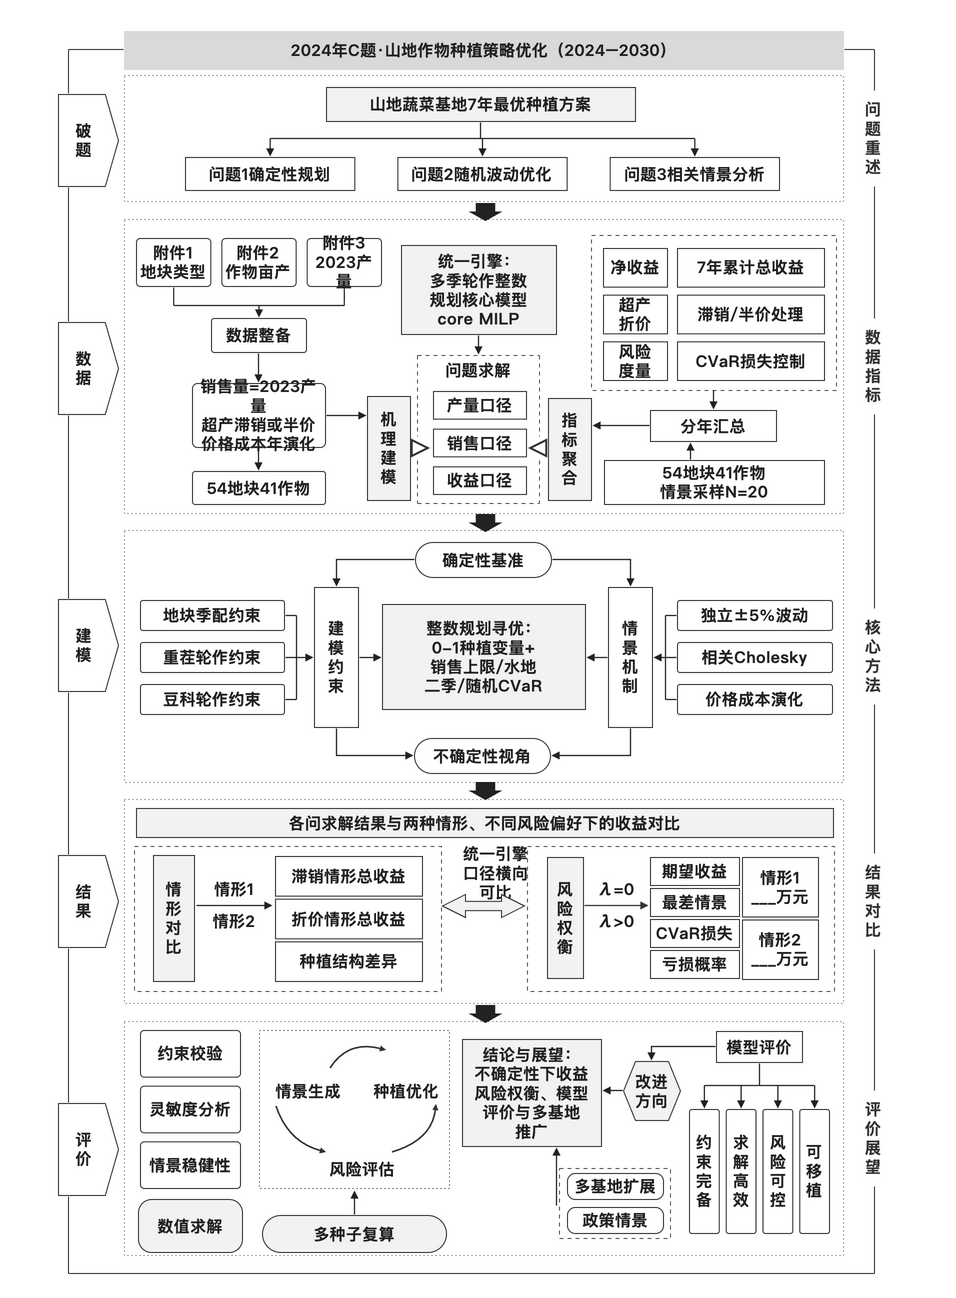
\includegraphics[width=0.80\textwidth]{figures/技术路线图.png}
	\caption{整体技术路线图}
	\label{fig:overall-technical-route}
\end{figure}

如图~\ref{fig:overall-technical-route} 所示，本文总体技术路线为：先对附件数据进行清洗与结构化，明确54地块41作物的容量、季节、轮作与销售约束；问题1在确定性口径下建立0-1整数规划模型，分别求解滞销与折价两种情形；问题2引入销售量、亩产量、价格的不确定性，建立基于情景模拟的两阶段随机规划模型，并用CVaR刻画尾部风险；问题3进一步刻画作物间替代、互补及产销联动相关结构，用Cholesky分解生成相关情景，分析相关结构对最优策略的影响。各问结果统一给出种植方案与收益、风险指标并进行横向对比。
